\documentclass[letterpaper, 8pt]{extarticle}
\usepackage{amssymb,amsmath,amsthm,amsfonts}
\usepackage{multicol,multirow}
\usepackage{calc}
\usepackage{ifthen}
\usepackage[landscape]{geometry}
\usepackage[colorlinks=true,citecolor=blue,linkcolor=blue]{hyperref}
\usepackage{booktabs}
\usepackage{ulem}
\usepackage{enumitem}
\usepackage{tabulary}
\usepackage{graphicx}
\usepackage{siunitx}
\usepackage{tikz}
\usepackage{derivative}
\usepackage{svg}
\usepackage{listings}
\usepackage{color}
\usepackage{soul}
\usepackage{clrscode3e}


\ifthenelse{\lengthtest { \paperwidth = 11in}}
    { \geometry{top=.25in,left=.25in,right=.25in,bottom=.3in} }
	{\ifthenelse{ \lengthtest{ \paperwidth = 297mm}}
		{\geometry{top=1cm,left=1cm,right=1cm,bottom=1cm} }
		{\geometry{top=1cm,left=1cm,right=1cm,bottom=1cm} }
	}

\newenvironment{Figure}
  {\par\medskip\noindent\minipage}
  {\endminipage\par\medskip}

\pagestyle{empty}
\makeatletter
\renewcommand{\section}{\@startsection{section}{1}{0mm}%
                                {-1ex plus -.5ex minus -.2ex}%
                                {0.5ex plus .2ex}%x
                                {\normalfont\normalsize\bfseries}}
\renewcommand{\subsection}{\@startsection{subsection}{2}{0mm}%
                                {-1explus -.5ex minus -.2ex}%
                                {0.5ex plus .2ex}%
                                {\normalfont\small\bfseries}}
\renewcommand{\subsubsection}{\@startsection{subsubsection}{3}{0mm}%
                                {-1ex plus -.5ex minus -.2ex}%
                                {1ex plus .2ex}%
                                {\normalfont\tiny\bfseries}}
\makeatother
\setcounter{secnumdepth}{0}
\setlength{\parindent}{0pt}
\setlength{\parskip}{0pt plus 0.5ex}
% -----------------------------------------------------------------------
% \tymin=37pt
% \tymax=\maxdimen

% Custom siunitx defs
\DeclareSIUnit\noop{\relax}

\NewDocumentCommand\prefixvalue{m}{%
\qty[prefix-mode=extract-exponent,print-unity-mantissa=false]{1}{#1\noop}
}

% Shorthand definitions
% \newcommand{\To}{\Rightarrow}

% condense itemize & enumerate
\let\olditemize=\itemize \let\endolditemize=\enditemize \renewenvironment{itemize}{\olditemize \itemsep0em}{\endolditemize}
\let\oldenumerate=\enumerate \let\endoldenumerate=\endenumerate \renewenvironment{enumerate}{\oldenumerate \itemsep0em}{\endoldenumerate}

\title{2GA3}

\begin{document}

\raggedright
\tiny

\begin{center}
	{\textbf{2GA3}} \\
\end{center}
\begin{multicols*}{4}
	\setlength{\premulticols}{1pt}
	\setlength{\postmulticols}{1pt}
	\setlength{\multicolsep}{1pt}
	\setlength{\columnsep}{2pt}

	\section{Logic Basics}
	% \subsection{Physics}
	% \textbf{Ohm's Law:} $R = \frac{U}{T}$\\
	% \textbf{Series:} \\
	% $R_T = \sum_{i=1}^N R_i$ \\
	% $V_T = \sum_{i=1}^N V_i$ \\
	% $I_T = I_1 = I_2 = \dots = I_N$\\
	% \textbf{Parallel:} \\
	% $1/R = \sum_{i=1}^N (1/R_i)$\\
	% $V_T = V_1 = V_2 = \dots = V_N$\\
	% $I_T = \sum_{i=1}^N I_i$ \\

	\subsection{Transistors}
	% REVIEW: Do we want an image here?
	MOSFETs have 4 components: Source, Gate, Drain, and Base

	\textbf{PNP/NMOS:} Is on when gate is positive. Does not have circle.\\
	\textbf{NPN/PMOS:} Is on when gate is negative. Has circle.

	Generally, transistors are used to pull the output to either
	a positive voltage, or a zero voltage (1 or 0, on or off).
	If output is not pulled to one of these,
	the output is floating and is indeterminate in voltage.

	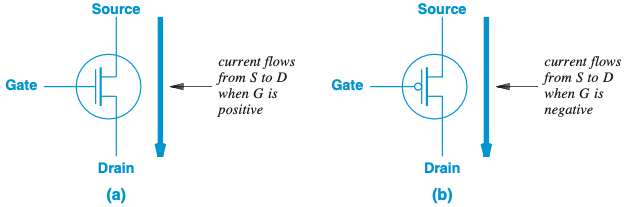
\includegraphics[width=\linewidth]{transistor-types.png}

	\subsection{Logic Circuits}
	\subsubsection{Symbols}

	\begin{center}
		\begin{tabular}{llllllll}
			\hline
			\multicolumn{1}{|l|}{p} & \multicolumn{1}{l|}{q} & \multicolumn{1}{l|}{and} & \multicolumn{1}{l|}{nand} & \multicolumn{1}{l|}{or} & \multicolumn{1}{l|}{nor} & \multicolumn{1}{l|}{xor} & \multicolumn{1}{l|}{invert p} \\ \hline
			1                       & 1                      & 1                        & 0                         & 1                       & 0                        & 0                        & 0                             \\
			1                       & 0                      & 0                        & 1                         & 1                       & 0                        & 1                        & 0                             \\
			0                       & 1                      & 0                        & 1                         & 1                       & 0                        & 1                        & 1                             \\
			0                       & 0                      & 0                        & 1                         & 0                       & 1                        & 0                        & 1
		\end{tabular}
	\end{center}

	% REVIEW: No clue if these are readable, needs to be printed
	% and double checked before release
	\begin{center}
		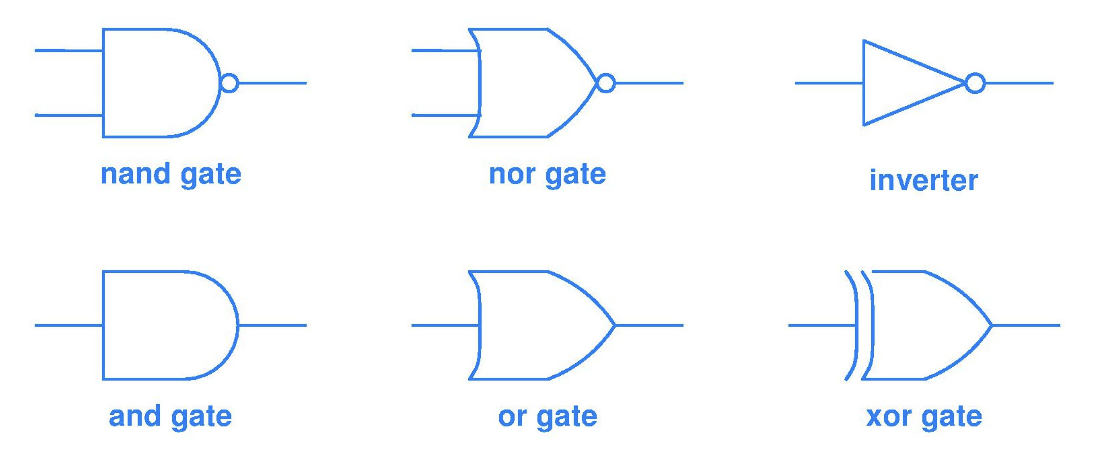
\includegraphics[width=.8\linewidth]{logic-gates.png}
	\end{center}
	\subsubsection{Adders}
	\begin{center}
		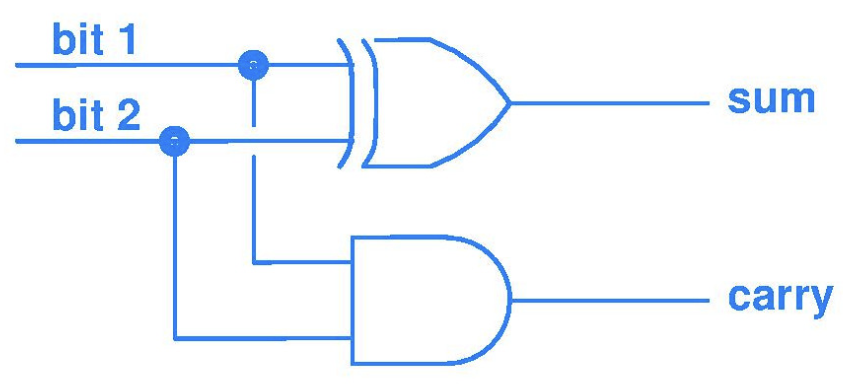
\includegraphics[width=.3\linewidth]{half-adder.png}
		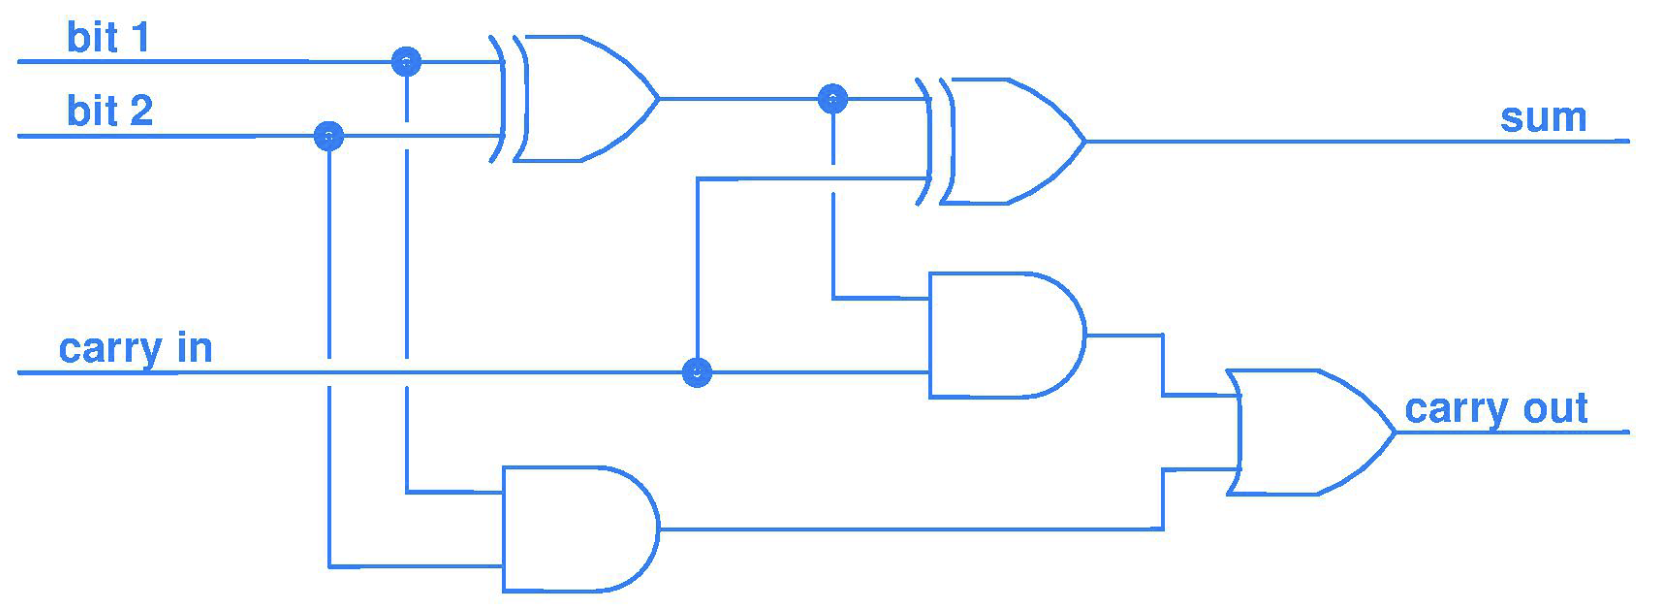
\includegraphics[width=.6\linewidth]{full-adder.png}
		Left: Half-adder. Right: Full-adder.
		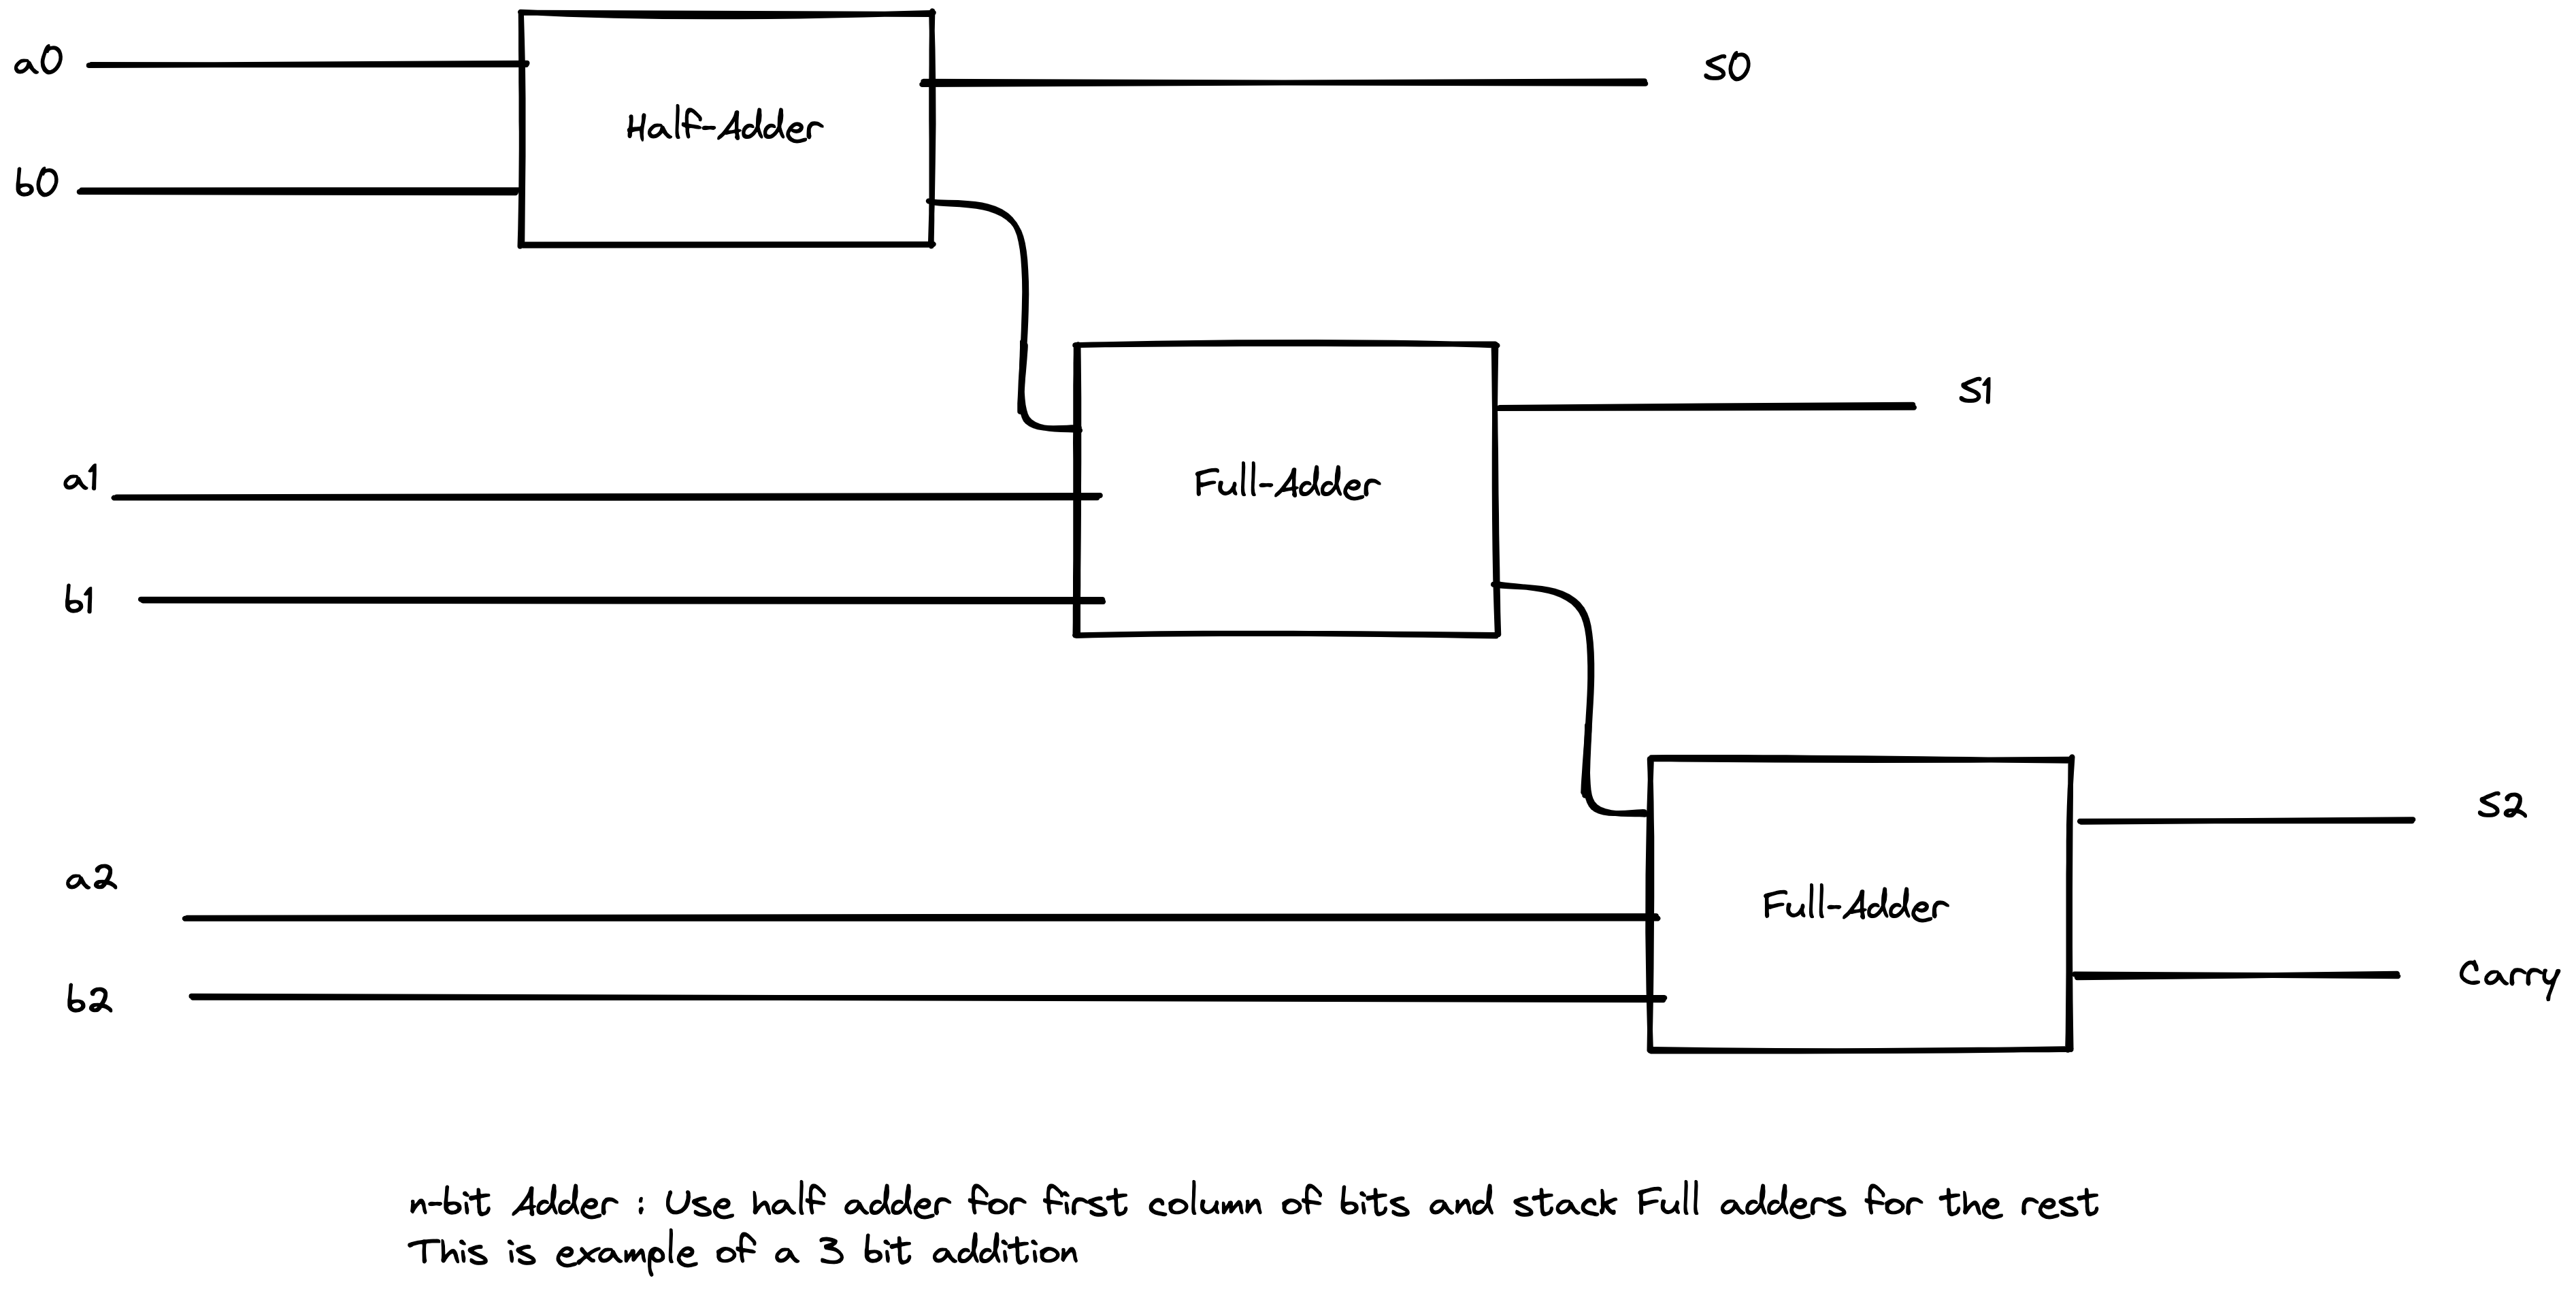
\includegraphics[width=0.8\linewidth]{n-adder.png}
	\end{center}
	% REVIEW: Is there anything else that needs to be added here?
	Half adders have no way to carry input from previous sums.
	To add more bits, just chain multiple full-adders together using the carry-out
	bit.
	If final carry at end is 1, that signifies an overflow error.

	\subsubsection{Latches \& Flip-flops}
	\textbf{Flip-flop}
	Every time the input switches from 0 to 1, the output switches to the opposite.
	% TODO: Add more detail about flip-flops

	\textbf{Gated D-latch}
	\begin{center}
		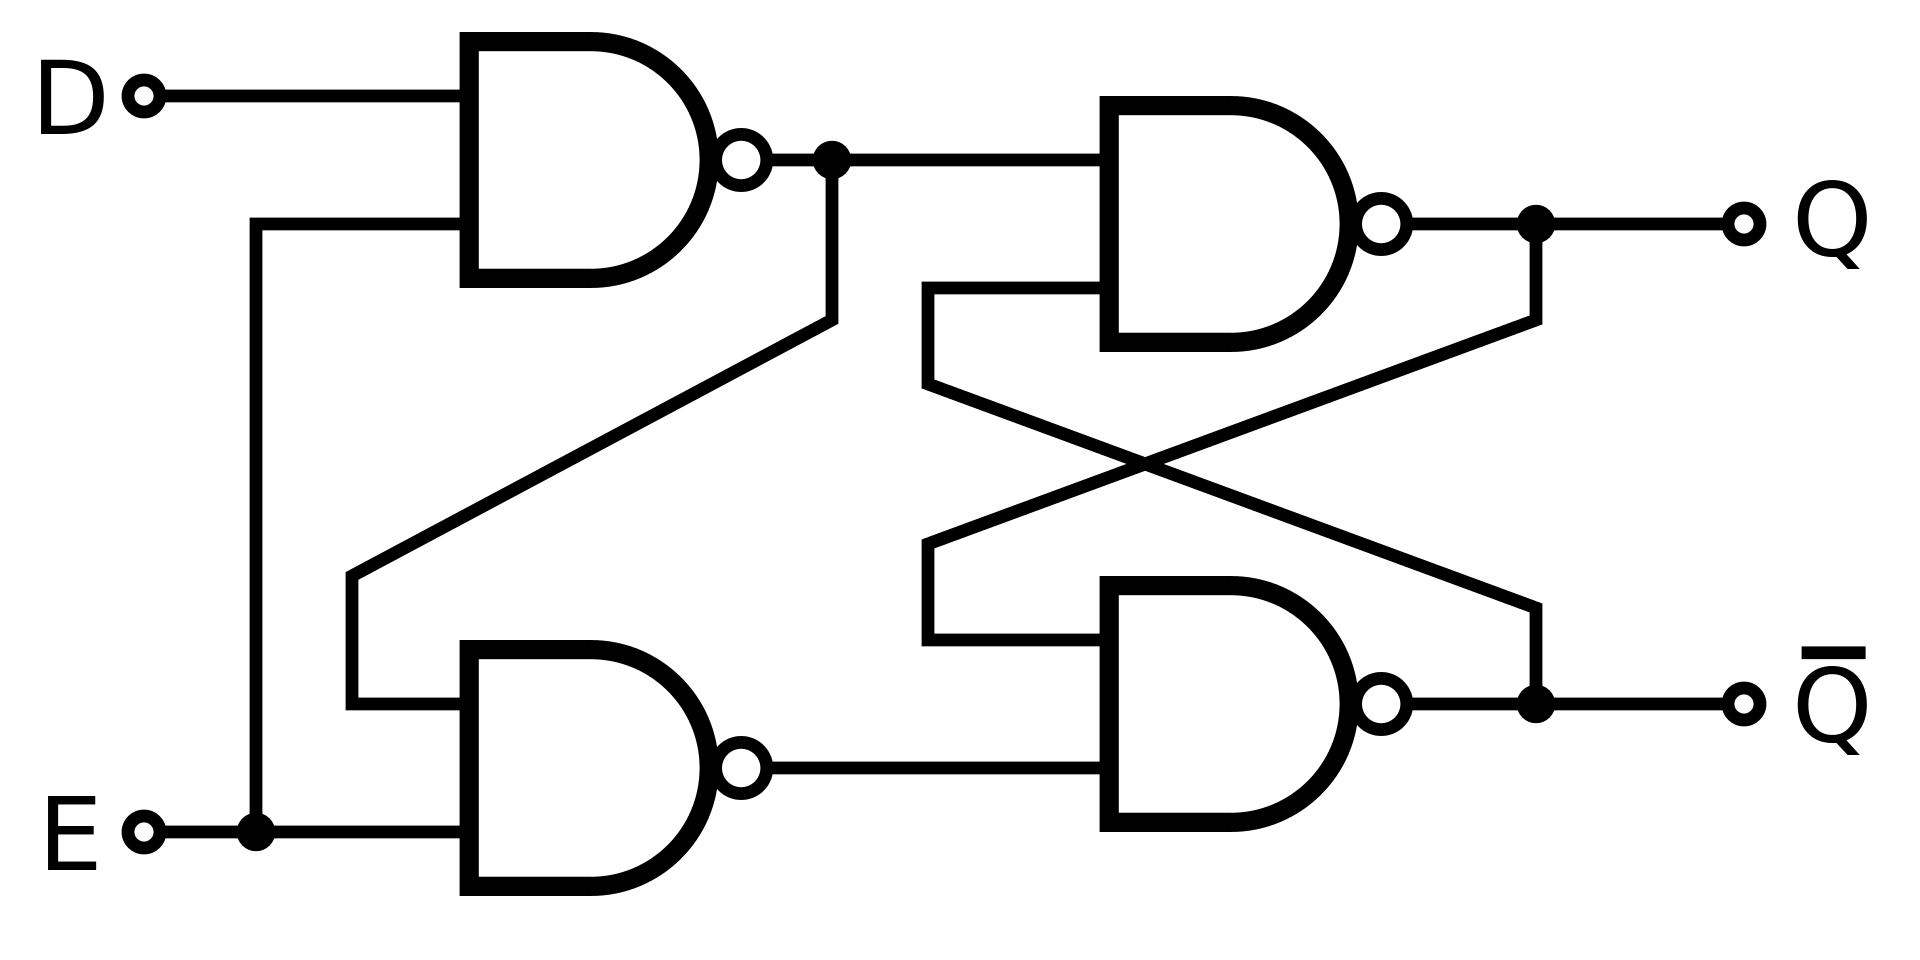
\includegraphics[width=.6\linewidth]{gated-d-latch.png}
		\begin{tabular}[!ht]{@{}cc|ccc@{}}
			\toprule
			$E/C$ & $D$ & $Q$               & $\overline{Q}$               & Comment   \\
			\midrule
			0     & X   & $Q_\textit{prev}$ & $\overline{Q}_\textit{prev}$ & No change \\
			1     & 0   & 0                 & 1                            & Reset     \\
			1     & 1   & 1                 & 0                            & Set       \\
			\bottomrule
		\end{tabular}
	\end{center}
	Operate on the principle of propagation delay.

	% REVIEW: Do we need this?
	% seems like a lot of space dedicated to something that's trivial to derive
	% from scratch
	Stacking many of them can be used to create a register:
	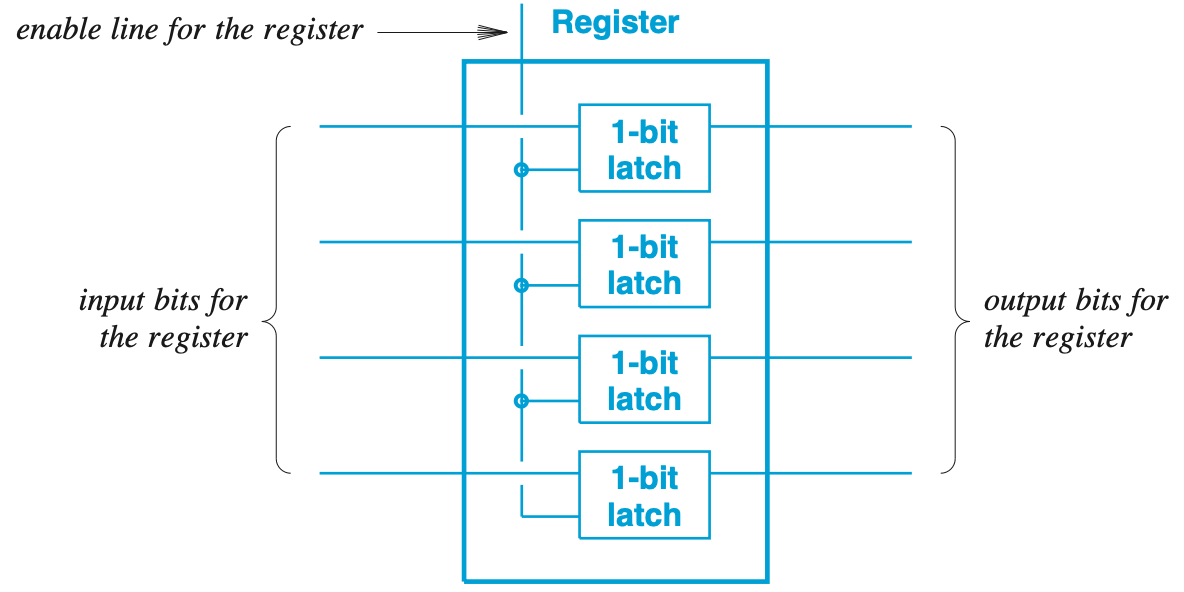
\includegraphics[width=\linewidth]{register.png}

	\subsection{Counters}
	For each transition from \textbf{low to high}, the counter increments the binary output by 1.
	(Counting the transition from high to low does the same thing, but the lecture used rising-edge counters).

	\subsection{Decoders}
	Take in an $n$-bit number, and turn on one of $2^n$ outputs.

	\subsection{Multiplexer / Demultiplexer}
	Multiplexer turns $n$ signals into a single signal, and Demultiplexer does the opposite

	\subsection{Software vs Hardware Design}
	Unlike software, which uses iteration, hardware uses replication. The advantages of replication are increased elegance, higher speed, and increased reliability.
	Hardware also uses gate minimization, abstraction and power optimization.

	\subsection{Fixed \& Programmable Logic}
	\textbf{Fixed logic circuits:} Pre-determined function.
	\textbf{Programmable logic:} FPGAs (reprogrammable, but still a significant cost to switching functions).
	\textbf{Stored program and re-programmable circuits:} Your computer right now.
	\section{Data Encoding}
	1 Byte = 8 bits.
	1 \textbf{Byte} encodes a character, integer, or pointer.
	1 \textbf{Word} is $n$ bytes, determined by the architecture.

	\subsection{Converting between bases}
	\textbf{Base 10 to Base N}
	Divide decimal \# by \# of new base.
	Take remainder as rightmost digit.
	Divide quotient of previous divide by new base.
	Repeat until quotient is zero.
	\textbf{Base N to Base 10}
	Take each column position of each digit, zero indexed, as $n$.
	For each column, do $c \cdot b^n$, where $c$ is the value of the column,
	and $b$ is the base value in base 10.

	\textbf{Important bases table}

	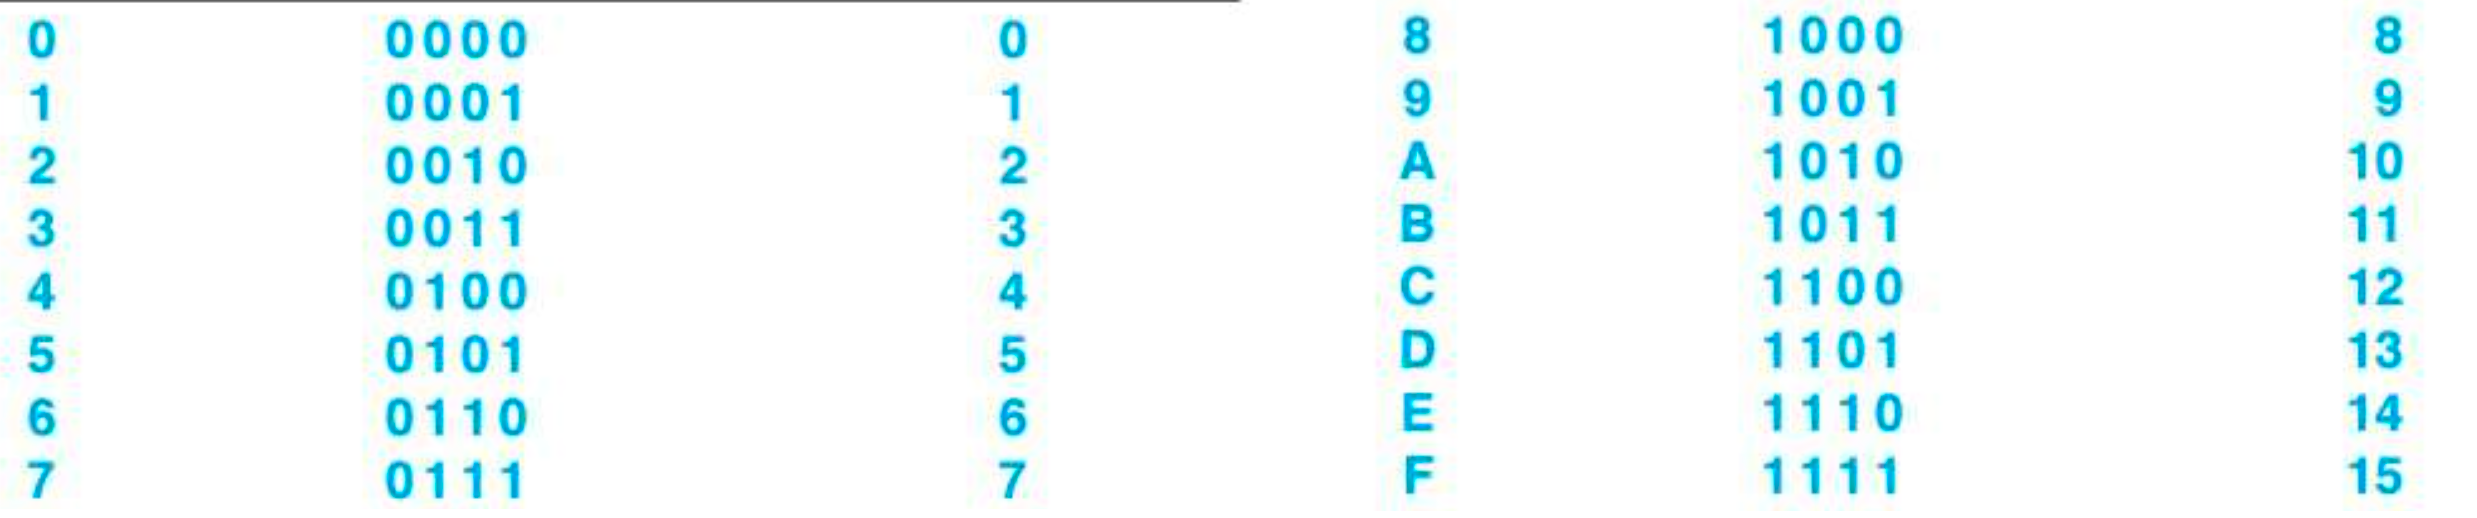
\includegraphics[width=.7\linewidth]{hex2bin.png}


	% REVIEW: if anyone can explain this better feel free to update this
	\subsection{Fraction to Binary}
	Convert integer part directly to binary, for fractional part, multiply fraction by 2 keeping notice of the resulting integer and fractional part. Continue multiplying by 2 until you get a resulting fractional part equal to zero. Then just write out the integer parts from the results of each multiplication.
	Eg : 3.375 = ? (binary)
	(0.375 * 2 = 0 + 0.75) (0.75 * 2 = 1 + 0.5)(0.5 * 2 = 1 + 0)
	Resuling binary will be 11.011
	\subsection{Signed Integers}
	\textbf{Sign-magnitude:} Dedicate one bit to the sign, and the rest to the magnitude.
	Range is $-(2^{n-1} - 1), +(2^{n-1} - 1)$, 0 sign means positive number,
	but has a positive and negative zero.
	\textbf{One's complement:} Invert all the bits to get negative number.
	Range is $-(2^{n-1} - 1), +(2^{n-1} - 1)$.
	\textbf{Two's complement:} Invert all bits, add a place value of 1 to get negative number.
	Eg, +6 is $0110$, so to get -6 go from $0110 \to 1001 \to 1010$.
	Range is $-(2^{n-1}), +(2^{n-1} - 1)$.

	\subsection{IEEE-754 Floats}
	Separated into \textbf{sign, exponent, and mantissa}.
	Entire float is represented in binary, and the exponent is biased by $2^{b-1} - 1$,
	where $b$ is the number of exponent bits.
	To calculate from IEEE, do $m_2 \times 2^{e_2}$.
	(Convert out of base 2 first).
	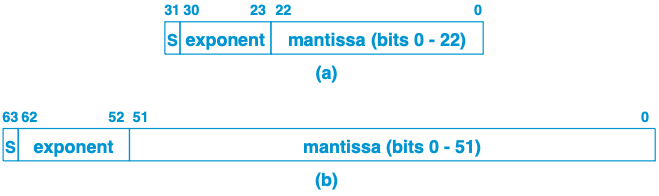
\includegraphics[width=\linewidth]{ieee-754.png}
	\subsubsection{Special Values}
	All bits being zero = zero.
	Exponent having all ones and mantissa having all zeroes = positive / negative infinity.
	Exponent having all ones and mantissa having something else = other error.


	\subsection{Types of architecture}
	\textbf{Von Neumann architecture:}
	\begin{itemize}
		\item Single memory block which contains both instructions and data.
		\item Offers complete flexibility: at any time, owner can change how much of the memory is devoted to programs and how much to data.
		\item More popular.
	\end{itemize}
	\textbf{Harvard architecture:}
	\begin{itemize}
		\item 2 separate memory. One is used for instruction, one is used for data.
		\item Inflexible, as u cannot use part of the instructional memory to store data and vise versa.
		\item Less popular. Sometimes used in small embedded systems.
	\end{itemize}

	\subsection{Types of processors}

	\textbf{Categories based on logic:} \\
	\begin{itemize}
		\item \textbf{Fixed logic}: Function fixed in hardware, performs a single task
		\item \textbf{Selectable logic}: Choose one of several fixed functions.
		\item \textbf{Parametrizable logic}: Accepts a set of parameters that control the computation of fixed functions.
		\item \textbf{Programmable logic}: list of instructions provided at runtime (you can code them)
	\end{itemize}

	\textbf{Categories based on Complexity:} \\
	\begin{itemize}
		\item \textbf{Co-processors}: Dedicated function. Usually performs a single task at high speed. Fixed/Selectable logic.
		\item \textbf{Microcontrollers}: Direct hardware control. Used in -> Elevator doors. Programmable logic.
		\item \textbf{Embedded System Processors}: real-time OS, dedicated hardware. usually more powerful than microcontrollers. Used in -> smart phone Programmable logic.
		\item \textbf{General-purpose Processors}: compatible for multiple systems. Used in -> CPU in a PC. Programmable logic.
	\end{itemize}

	\subsection{Parts of a processor}
	\begin{itemize}
		\item \textbf{Controller}: Responsible for program execution. Steps through the program and coordinates the actions of all other units.
		\item \textbf{Arithmetic logic unit}: Performs all computational tasks. Performs one operation at a time according to controller.
		\item \textbf{Local storage (registers)}: Hold data values such as operands for arithmetic operations and the result.
		\item \textbf{Internal connections}: Transfers data values between units, like from local storage to the ALU. AKA data paths/Bus/Control lines
		\item \textbf{External interface}: Handles all communication between the processor and the rest of the computer system.
	\end{itemize}

	\subsection{Fetch execute cycle}
	There is a \textbf{instruction pointer} which moves through the program performing every step. The cycle never ends while the system is runing.
	\begin{itemize}
		\item Fetch the next instruction
		\item Decode the instruction and fetch operands from registers
		\item Perform the arithmetic operation specified by the \textbf{opcode}
		\item Perform memory read or write, if needed
		\item Store the result back to the registers
		\item go to next instruction, Repeat forever.
	\end{itemize}

	\subsection{Program Translation}
	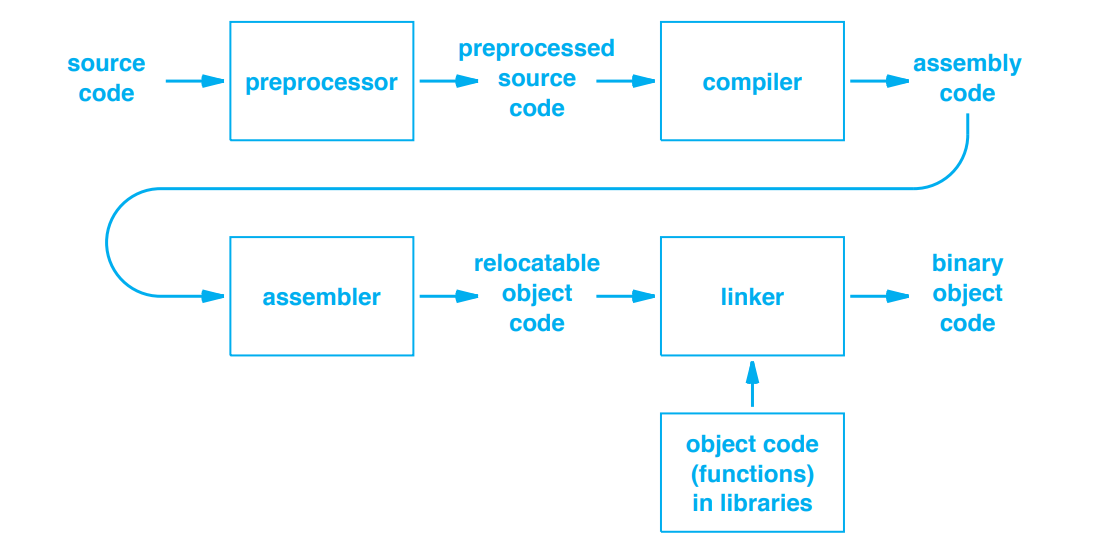
\includegraphics[width=\linewidth]{program-translation.png}
	\begin{itemize}
		\item \textbf{Preprocessor:} Expands macros, producing modified source program.
		\item \textbf{Compiler:} Translates it to assembly.
		\item \textbf{Assembler:} Translates it to relocatable object code which contains references to external library functions.
		\item \textbf{Linker:} Replaces external function references with its code.
	\end{itemize}

	\subsection{CISC vs RISC}
	\textbf{CISC}
	\begin{itemize}
		\item Each instruction performs a complex operation
		\item Instructions may take multiple clock cycles
		\item Fewer instruction calls
	\end{itemize}
	\textbf{RISC}
	\begin{itemize}
		\item Each instruction performs a simple operation
		\item Instructions all take the same number of clock cycles
		\item Many instruction calls needed
		\item Allows for pipelining, as each part of the instruction takes the same amount of time
	\end{itemize}

	\subsection{Pipelines}
	Allow for more than one instruction to be ``processed'' at the same time.
	By moving instructions through a pipeline, non-conflicting parts of an instruction
	can be worked on in steps.
	Generally 5 stages: Fetch next instruction, decode \& fetch operands,
	perform arithmetic operation, read or write memory, store result.

	\subsubsection{Pipeline Stalls}
	Also known as hazards. 3 main types:
	\textbf{Data Hazards:} Waiting for data from an earlier instruction.
	Instruction must wait before fetching operands,
	and can only complete that stage on the same cycle that the dependance is in the done stage.
	% REVIEW: Explanation for the line above is worded kinda poorly, if anyone wants to fix it up.
	Can be dealt with using data forwarding (allowing data to be used before it exits the pipeline),
	re-arranging instruction order.
	\textbf{Control Hazards:} Incorrect instruction is in the pipeline (branching).
	Can be dealt with using conditional branch prediction, flushing pipeline if prediction is wrong.
	\textbf{Structural Hazards:} Resource conflict (eg accessing the same register bank).
	Can be dealt with by loading data in parallel, eg using multiple banks.

	\subsection{Branching}
	Moving the instruction pointer to a different location in program.
	Can be either absolute branch, or relative branch.
	% REVIEW: idk what else needs to be added here,
	% this seems pretty trivial

\end{multicols*}

\end{document}